\newpage
\chapter{Logica CMOS}

La logica tuttora utilizzata è la cosiddetta logica di tipo CMOS: complementary metal-oxide semiconductor.

Il problema della logica a rapporto è che quando l'uscita è a zero, il pull-down conduce, ma anche il pull-up conduce e c'è uno \textbf{spreco} di corrente. 

Un modo per risolvere la situazione è fare in modo che quando l'uscita deve andare a zero, il pull-down conduca ma il pull-up no, si deve staccare. Questa è la logica CMOS.

\paragraph{}
Infatti essa utilizza in maniera simmetrica i transistori nMOS e pMOS, simile all'inverter pseudo pMOS.


\begin{figure}[htbp]
    \centering
    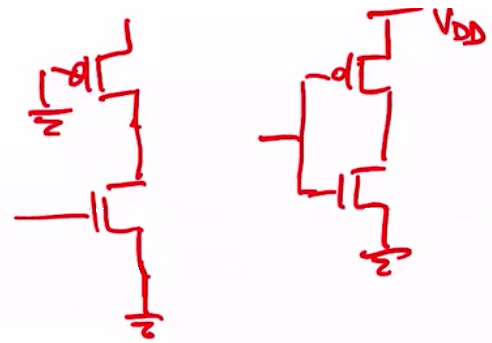
\includegraphics[width=0.25\linewidth]{img/pseudo_inv_e_CMOS.png}
    \caption{Pseudo nMOS a sinistra, logica CMOS a destra}
    
\end{figure}

Nella logica CMOS anche il pMOS funzione da interruttore invece che da carico.


\begin{figure}[htbp]
    \centering
    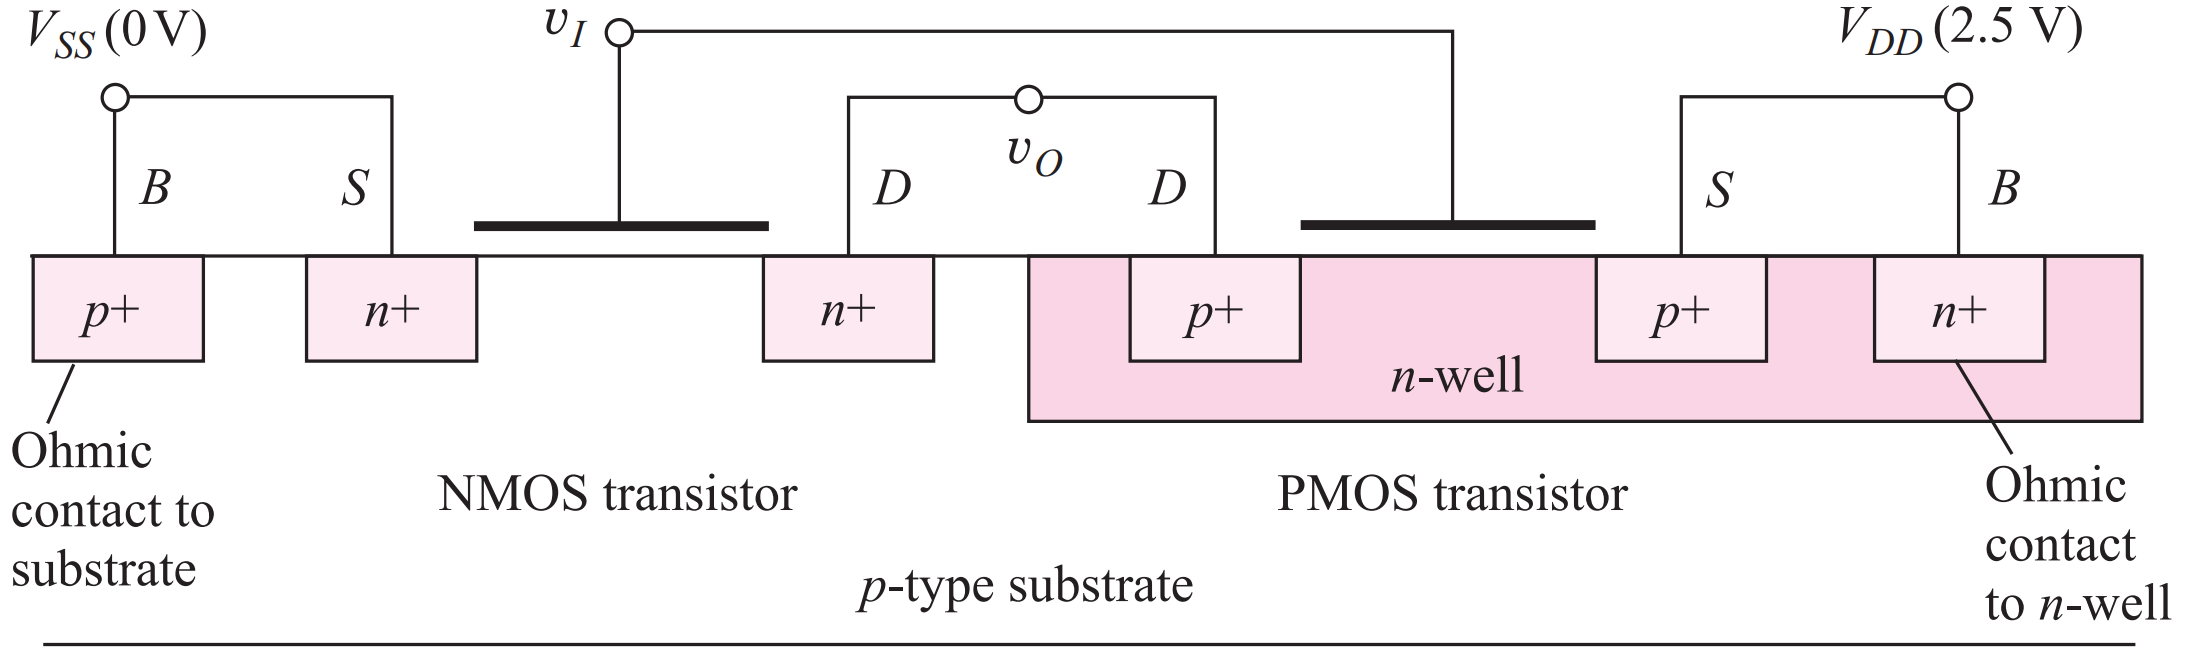
\includegraphics[width=0.60\linewidth]{img/CMOS.png}
    \caption{Logica CMOS}
    
\end{figure}

Si vede che con questa logica quando l'ingresso è alto, il pMOS si stacca e l'nMOS non ha nessuno con cui competere; quando l'ingresso è basso, invece, è l'nMOS che si stacca. Logica appunto \textbf{complementare}.

\paragraph{Perché allora la logica CMOS non viene usata anche per costruire l'inverter?} Perché si complicherebbe pure il pull-up, creando dunque un circuito più grande. Soprattutto se si pensa a funzioni logiche complicate.

Ad esempio una NAND a tre ingressi nella logica a CMOS avremo 6 transistori; mentre nella logica a rapporto avremo solamente 4 transistori, dato che il pull-up non cambia.

\newpage
\section{Inverter CMOS}

Entrambi i transistori controllati da	tensione di	ingresso, attivi in fasi differenti e funzionamento simmetrico. I parametri non sono completamente simmetrici.


\begin{figure}[htbp]
    \centering
    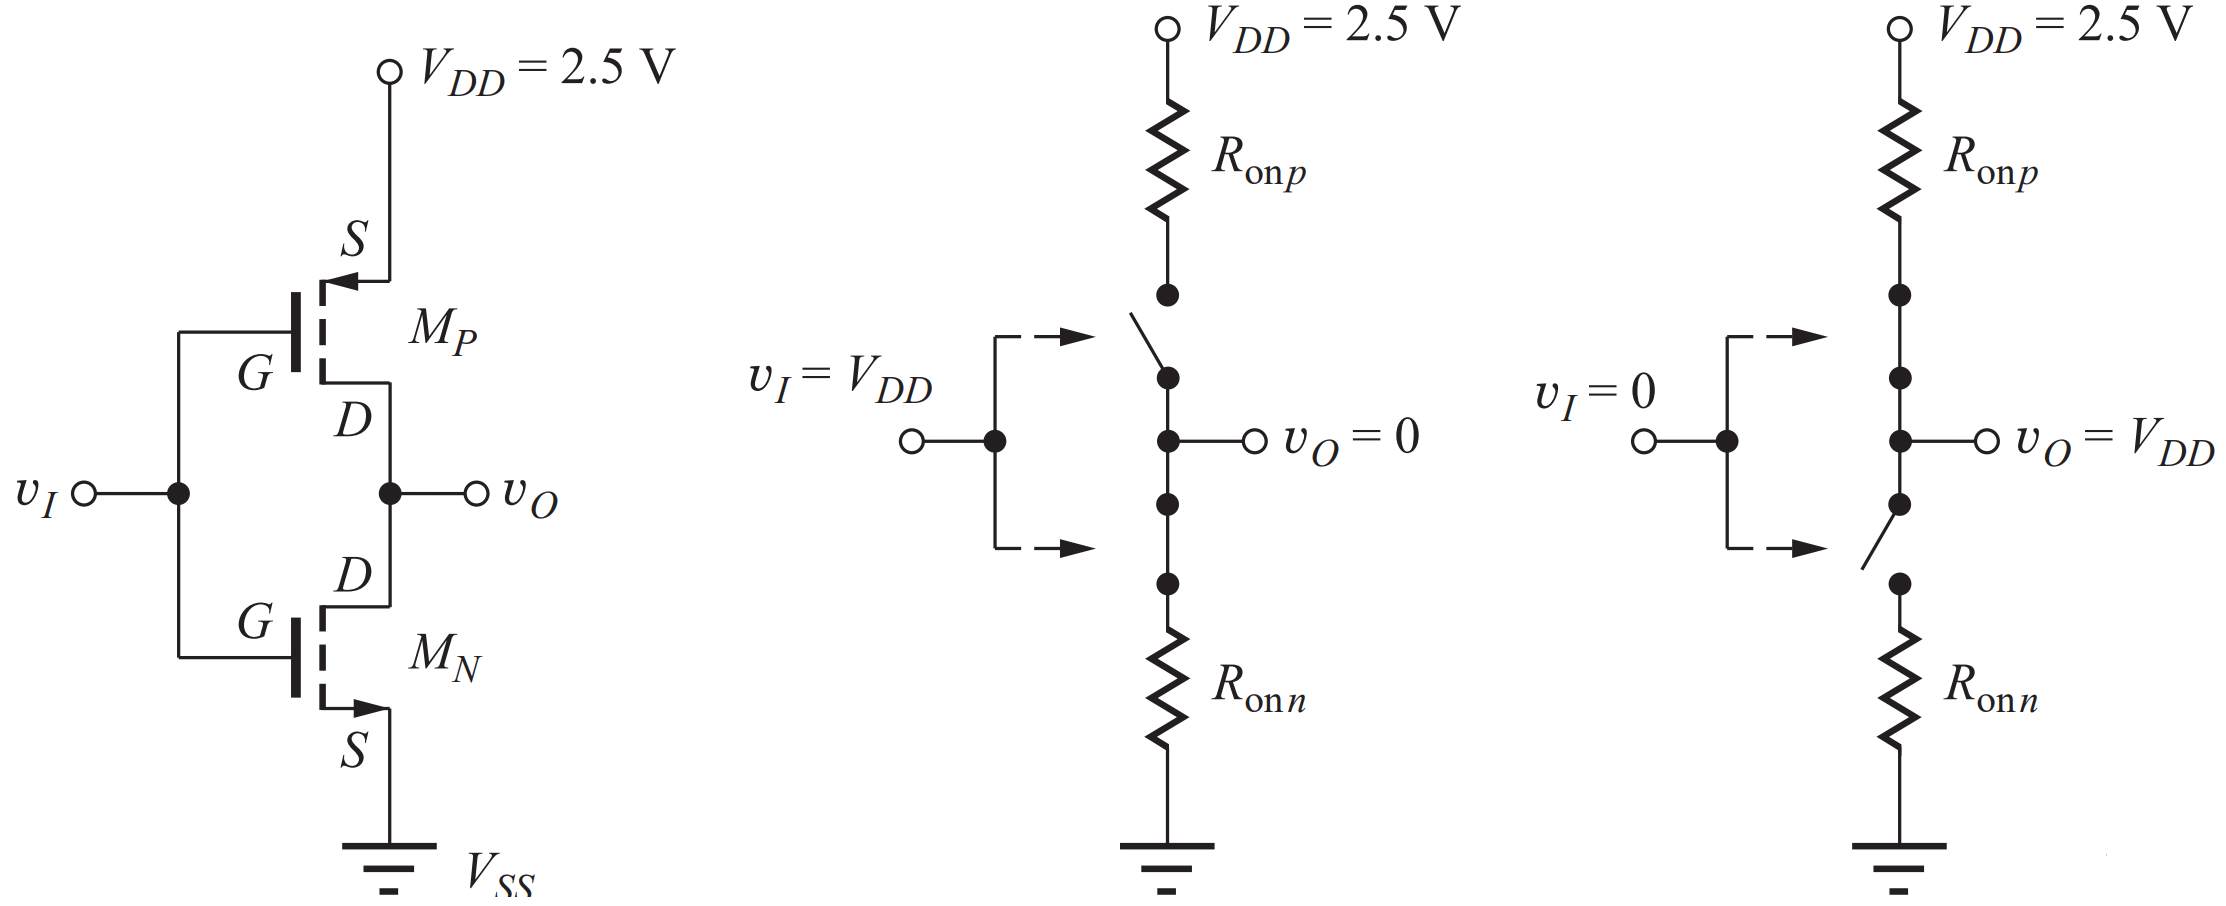
\includegraphics[width=0.65\linewidth]{img/inveerrter_CMOS.png}
    \caption{Inverter CMOS}
    \label{Inverter_cmos}
\end{figure}

In questa maniera, prima avevamo dimensionato il circuito tale per cui l'uscita andava a $0.2\,V$, ora invece l'uscita può andare proprio a $0\,V$, e non ci sarà nessuna competizione (partitore di tensione).

\paragraph{}
L'uscita non dipende dalle dimensioni, rapporto $\frac{W}{L}$, dei transistori, bensì si possono fare tutti della \textbf{dimensione minima}. Il rapporto varia solo la transconduttanza, contiene sempre il rapporto, e dunque influenza la resistenza, quest'ultima influisce sulle tempistiche e ora il dimensionamento si può fare sulle tempistiche al posto che sui livelli, che in CMOS sono o $0\,V$, oppure $V_{DD}$.

Inoltre si migliorano pure i margini di rumore, dato che utilizziamo tutta l'escursione e non solo una parte.


\paragraph{NOTA:} Per capire quale è il pMOS e l'nMOS si guarda la freccia della corrente. Nella Figura \ref{Inverter_cmos} la freccia che entra nel canale indica il pMOS, quella che esce indica il nMOS. Inoltre il tratteggiato indica un canale ad arricchimento, si deve creare lo strato; il non tratteggiato indica un transistore a svuotamento, il canale lo ha già e al limite lo si toglie abbassando la $V_{GS}$. Tutto ciò in elettronica digitale, essendo dispositivi ad arricchimento, per semplicità di disegno la linea del canale la si fa solida.

\subsubsection{Per $V_I = V_{DD}$}

\begin{itemize}
    \item $V_{GS} =	V_{DD}$ per	nMOS,	che conduce	e	scarica la	capacità C
    \item $V_{GS} =	0$	per	pMOS,	che quindi si trova in	regione di	cut-off	e non	conduce	corrente
    \item La	tensione di	uscita finale	$VL =	0$
\end{itemize}


\paragraph{Nota:} inizialmente il transistore nMOS è in	saturazione,	quando l'uscita è ancora alta e man	mano che C	si scarica,
si passa alla zona triodo.

\subsubsection{Per $V_I = 0$}

\begin{itemize}
    \item $V_{GS} =	-2.5$ per	pMOS,	che conduce	e	carica la	capacità C
    \item $V_{GS} =	0$	per	nMOS,	che quindi si trova in	regione di	cut-off	e	non	conduce	corrente
    \item La	tensione di	uscita finale	$VL =	V_{DD}$
\end{itemize}

\paragraph{Nota:}	inizialmente il transistore pMOS è in	saturazione,	quando l'uscita è ancora bassa e man	mano che C	si carica, si passa alla zona triodo.

\newpage
\section{Vantaggi dei CMOS}

\begin{itemize}
    \item Lo	0	e	1	logico corrispondono alle tensioni di	alimentazione, dunque ci aspettiamo che margini di	rumore saranno grandi;
    \item I	livelli non	dipendono dalle dimensioni dei transistori, si	possono fare	entrambi delle dimensioni minime a	vantaggio dell'area;
    \item Sia lo	0	che 1	logico sono pilotati direttamente, bassa impedenza di	uscita ($\approx K\Omega$, o meno),	alta immunità ai disturbi
    \item Alta	impedenza di	ingresso, ogni porta	può pilotare moltissime altre porte
    \item Consumo statico di	potenza nulla, regime	non	c'è un	flusso di	corrente tra $V_{DD}$ e	massa, solo	consumo dinamico (in	prima	approssimazione)
\end{itemize}

\subsubsection{Caratteristica statica in tensione}

La caratteristica è derivabile incrociando le caratteristiche I-V dei due transistori, imponendo che le correnti di drain siano uguali si individuano precise	zone	di	funzionamento per	i due	 transistori. Dimensioniamo i transistori in	modo che $K_P =	K_N$ per avere una simmetria.


\begin{figure}[htbp]
    \centering
    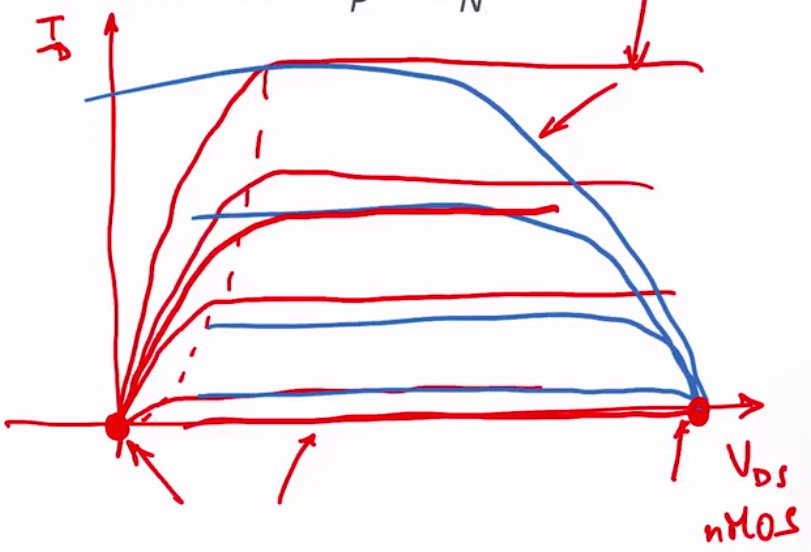
\includegraphics[width=0.44\linewidth]{img/caratt_cmos.png}
    \caption{Caratteristica statica in tensione CMOS}    
\end{figure}

Partendo dal nMOS alto e pMOS basso, man mano che aumenta l'ingresso la tensione sul nMOS scende mentre aumenta quella del pMOS.

\newpage
\subsection{Ingresso zero}

\begin{figure}[htbp]
    \centering
    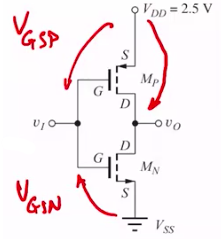
\includegraphics[width=0.25\linewidth]{img/casdb.png}
    
\end{figure}

L'nMOS è in cut-off, dato che la sua $V_{GS} = 0\,V$. Mentre il pMOS conduce e l'uscita conduce alla tensione di $V_{DD}$.

\begin{figure}[htbp]
    \centering
    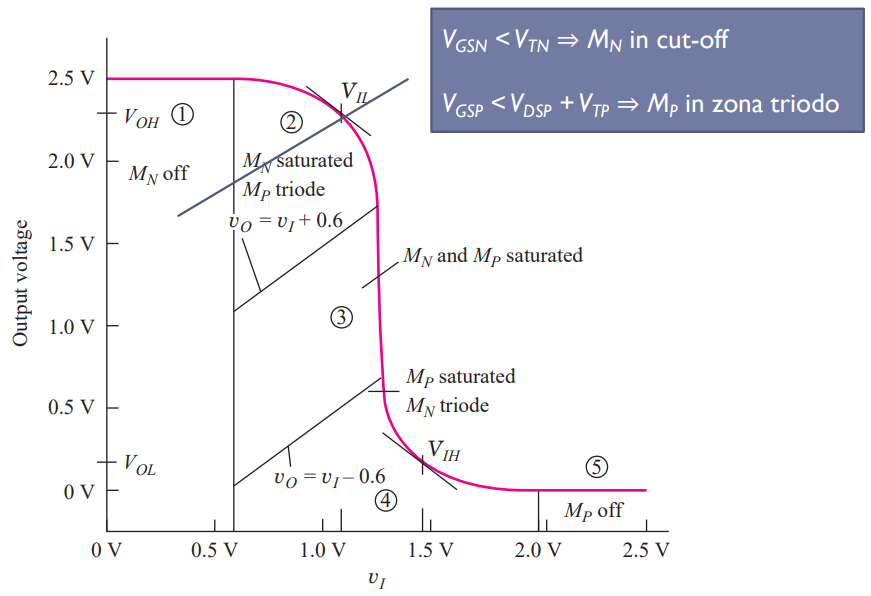
\includegraphics[width=0.7\linewidth]{img/zona_1.png}   
    
\end{figure}


\newpage
\subsection{Accensione dell'nMOS}

Aumentando l'ingresso la $V_{GSP}$ diminuirà, in valore assoluto avvicinandosi alla sua soglia ($-0.6\,V$) ancora molto lontana per il momento. Quando infatti arriviamo ad un ingresso di $0.6\,V$ l'nMOS si attiva, in questa fase di transizione entrambi i transistori sono in conduzione, il pMOS continua ad essere in zona triodo ($-2.5+0.6\,V = -1.9\,V$) molto al di sotto della soglia di $-0.6\,V$.


Mentre l'nMOS, accendendosi, si ritrova l'uscita alta ma il suo ingresso è appena sopra la soglia e non siamo dunque una soglia sopra l'uscita, per questo motivo ci troviamo in saturazione.

\paragraph{}
Aumentando sempre più l'ingresso il pMOS condurrà di meno, viceversa per l'nMOS e l'uscita scende.

\begin{figure}[htbp]
    \centering
    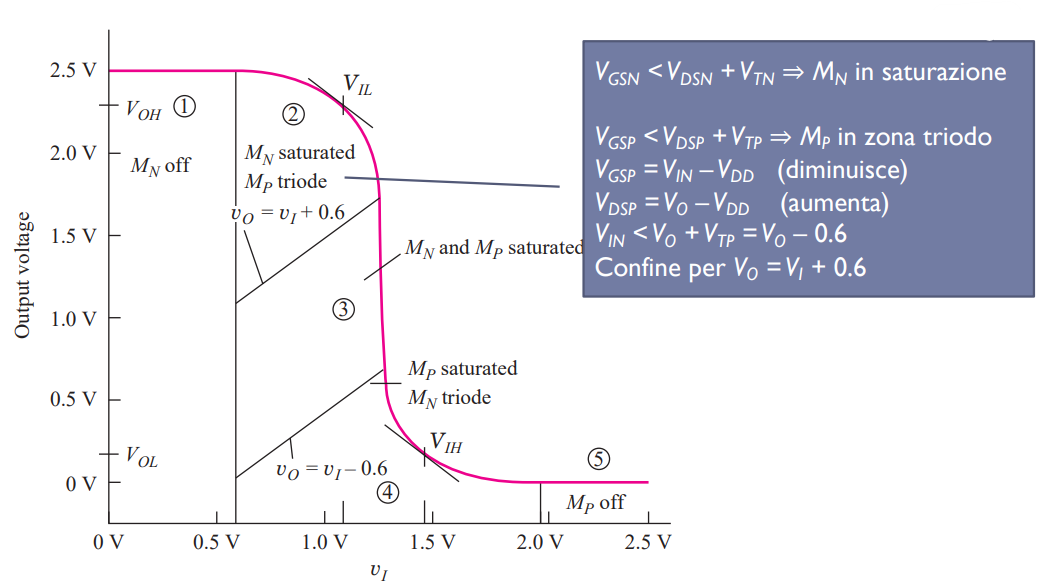
\includegraphics[width=0.8\linewidth]{img/zona_2.png}  
    
\end{figure}


\subsection{Aumentiamo ancora l'ingresso}

Siamo per entrambi i transistori in zona di saturazione e stanno tirando in modo simile, siamo alla commutazione. Aumentando ancora l'ingresso possiamo far entrare in zona triodo il transistore nMOS.


\begin{figure}[htbp]
    \centering
    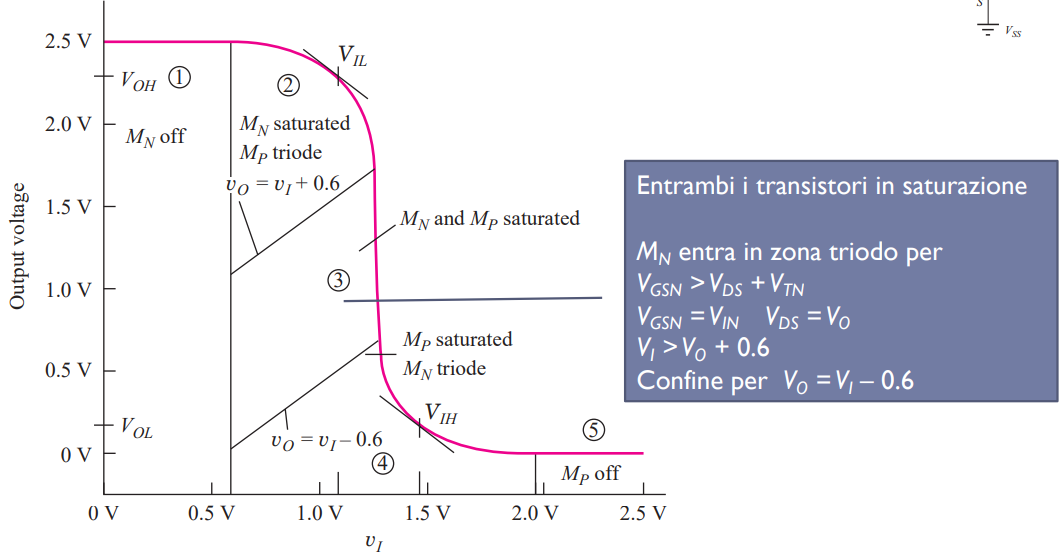
\includegraphics[width=0.85\linewidth]{zona_3.png}
\end{figure}


\newpage
\subsection{Zona triodo nMOS}

Aumentando ancora l'ingresso a questo punto la $V_{GSN}$ supererà di una tensione di soglia l'uscita e passerà in zona triodo, con il pMOS in zona di saturazione.

Con l'nMOS che tira di più, la corrente è sempre la stessa però tira l'uscita a massa.

\begin{figure}[htbp]
    \centering
    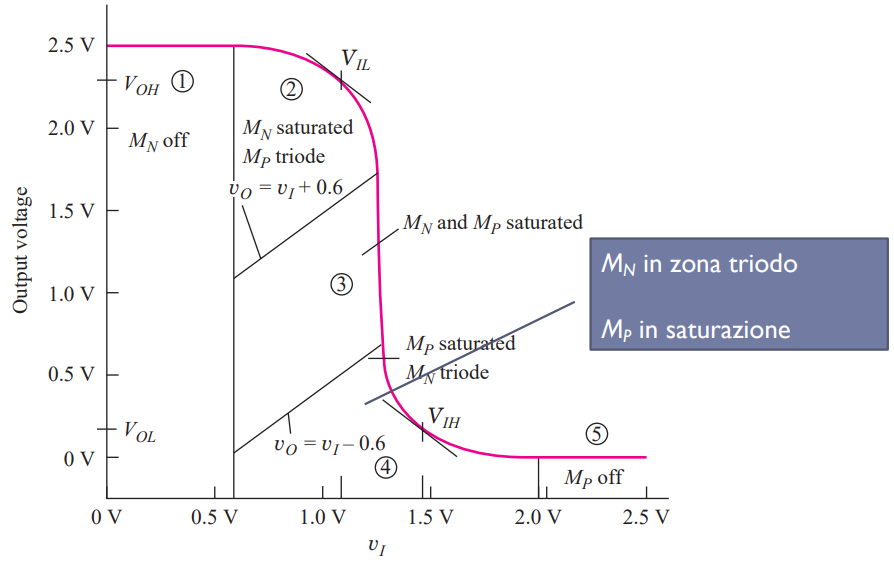
\includegraphics[width=0.75\linewidth]{img/zona4.png}
    
    
\end{figure}


\subsection{Zona cut-off pMOS}

Il pMOS si spegnerà quando la sua $|V_{GSP}| < |0.6|\,V$, e a questo punto la tensione in uscita arriva effettivamente a zero.

\begin{figure}[htbp]
    \centering
    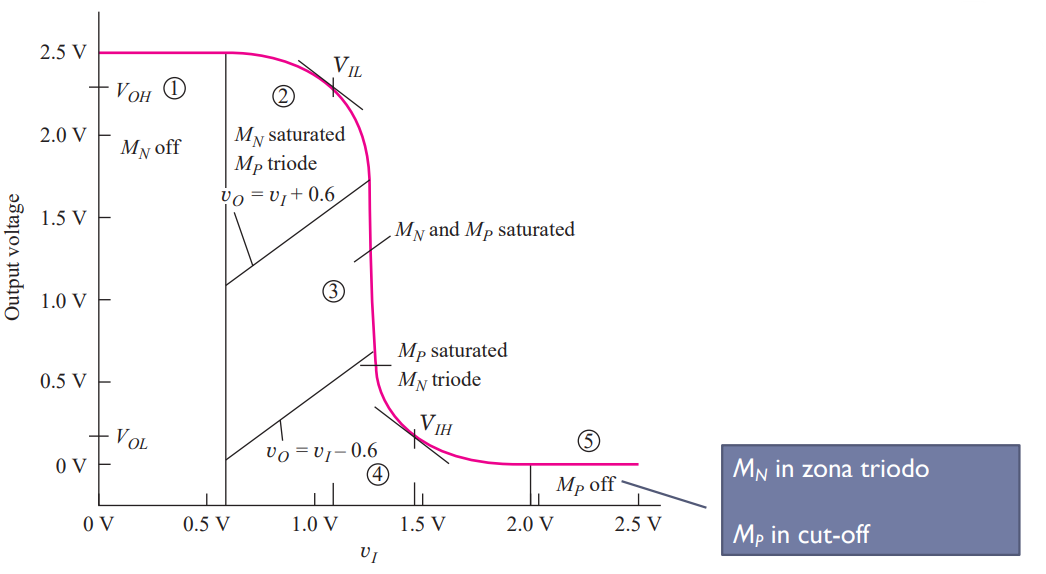
\includegraphics[width=0.85\linewidth]{img/ZONA5.png}
    
    
\end{figure}


Se consideriamo dei transistori senza modulazione di lunghezza di canale, la zona 3 risulta effettivamente molto verticale, questo perché le caratteristiche di pMOS e nMOS si sovrappongono. Mentre se si considera la modulazione di lunghezza di canale questa zona sarà meno verticale.


\newpage
\section{Rapporto tra n e p MOS}

Nel caso precedente le transconduttanza erano uguali, ma quest'ultima non è detto che siano uguali. Intanto le mobilità possono essere diverse e il rapporto $\frac{W}{L}$ anch'esso potrebbe variare.

\subsubsection{Comportamento simmetrico se $K_n = K_p$ }

Per ottenere questo valore basta uguagliare le transconduttanza:

\begin{equation*}
    K_n'\frac{W_n}{L_n} = k_p'\frac{W_p}{L_p} \qquad\to\qquad \frac{W_p}{W_n} = \frac{K_n'}{K_p'}\frac{L_p}{L_n}
\end{equation*}

Assumendo $L_p =L_n$

\begin{equation*}
    K_p' = 40,\, K_n' = 100 \qquad\to\qquad W_p = 2.5W_n
\end{equation*}

Normalmente si fa una $W_p$ più grande per compensare il fatto che le lacune hanno una mobilità inferiore, e dunque la corrente del p è inferiore a n.

\subsubsection{Asimmetria}

\begin{equation*}
    K_R = \frac{K_n}{K_p}
\end{equation*}

\begin{figure}[htbp]
    \centering
    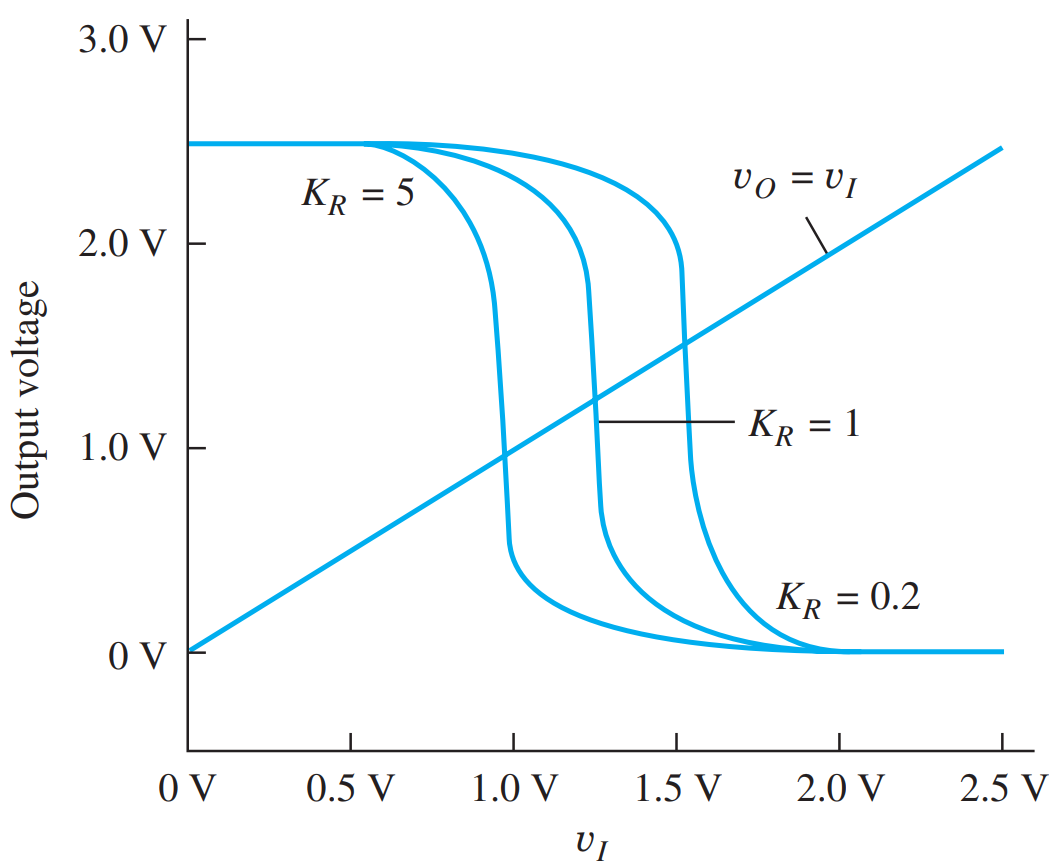
\includegraphics[width=0.55\linewidth]{img/asimmetria.png}
    \caption{Asimmetria}    
\end{figure}

Spesso si cerca di farla simmetrica, ma non è detto infatti spostare la caratteristica si spostano i valori $V_{OH}$ e $V_{OL}$ e questo cambia i valori di margine di rumore. Se simmetrico i due margini sono uguali, mentre se è asimmetrico si diminuisce e contemporaneamente aumenta il margine di 1 o 0.

\newpage
\section{Margini di rumore}

\subsection{$V_I = V_{IH}$}
Ipotizzando che l'ingresso si alto il pMOS è in saturazione, mentre l'nMOS è in zona triodo, le correnti di drain devono essere uguali:

 \begin{equation*}
     K_n\biggl(V_I - \vtn - \frac{V_O}{2}\biggl)V_O = \frac{K_p}{2}(VI -\vdd - V_{TP})^2
 \end{equation*}


 Risolvendo per $V_O$, e derivando rispetto a $V_I$ e uguagliando a $-1$ otterremo:

 \begin{equation*}
     V_{IH} = \frac{5\vdd + 3\vtn + 5V_{TP}}{8} \qquad\qquad\qquad V_{OL} = \frac{\vdd - \vtn + V_{TP}}{8}
 \end{equation*}

 \subsection{$V_I = V_{IL}$}

 Stessi passaggi visti prima ma in questo caso si applica quando l'ingresso è basso:

 \begin{equation*}
     V_{IL} = \frac{3\vdd + 5\vtn + 3V_{TP}}{8} \qquad\qquad\qquad V_{OL} = \frac{7\vdd - \vtn + V_{TP}}{8}
 \end{equation*}

Nel nostro caso i margini di rumore sono entrambi di $0.93\,V$, molto buoni se confrontati con l'inverter con logica a rapporto.

\section{Comportamento dinamico}

Supponiamo che l'ingresso passi dal valore basso al valore alto, l'nMOS si attiva e il pMOS si interdice e la capacità verrà scaricata.
\paragraph{}
Per calcolarla useremo la resistenza efficace dell'nMOS e  ipotizzando una scarica esponenziale.


\begin{figure}[htbp]
    \centering
    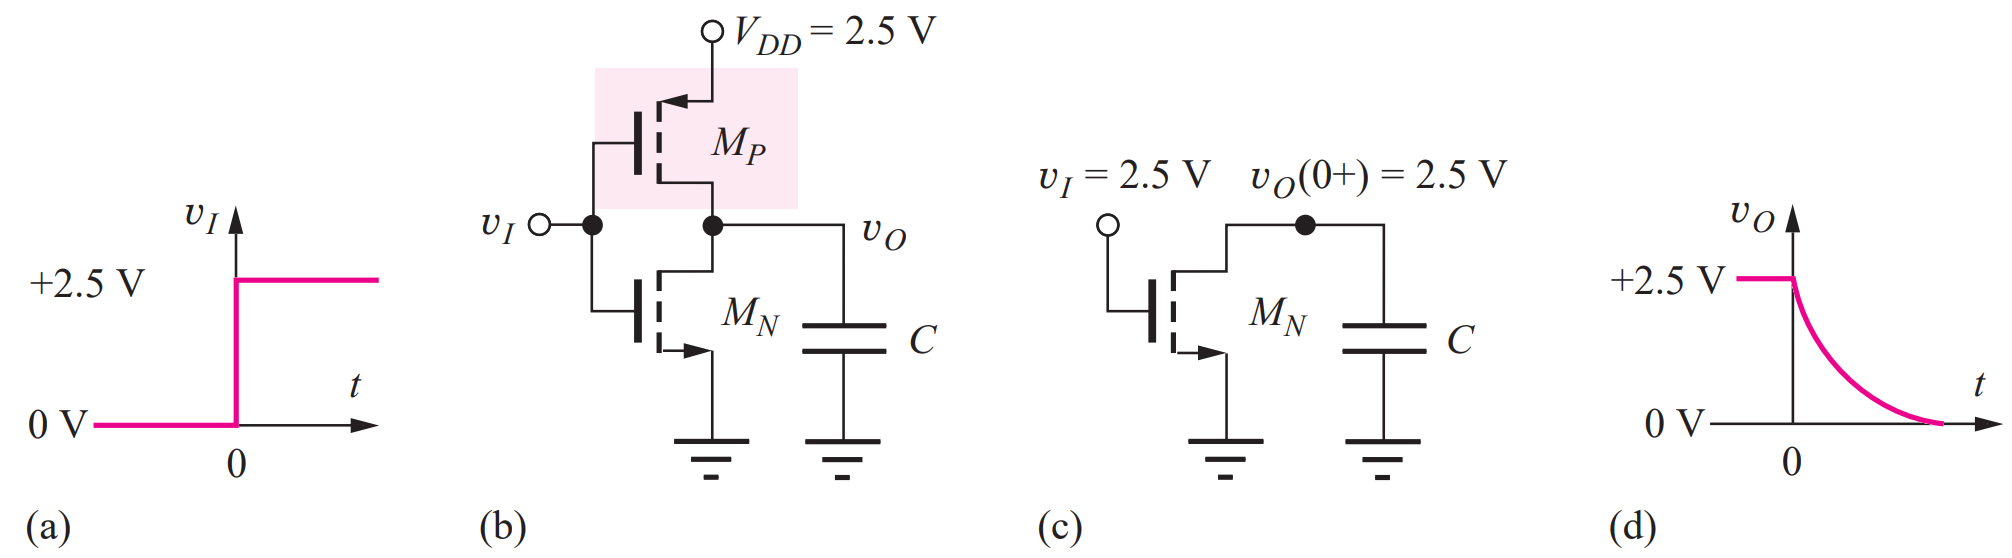
\includegraphics[width=0.95\linewidth]{img/dinamico.png}
    
    
\end{figure}


\subsection{Transitorio in discesa}

Funzionamento simile all'invertitore nMOS a carico resistivo, calcoliamo la resistenza equivalente dell'nMOS supponendo che questo sia in zona triodo:

\begin{equation*}
    R_{on} =\frac{1}{K_n(\vgs - \vt)}
\end{equation*}

Dobbiamo aggiustarlo per un fattore, dato che all'inizio la corrente è costante:

\begin{equation*}
    R = 1.7R_{on}
\end{equation*}

\subsection{Tempo di discesa:}

\begin{equation*}
    t_f = 2.2(1.7R_{on}C) = 3.7R_{on}C
\end{equation*}

\subsection{Tempo di propagazione da alto a basso dell'uscita:}

\begin{equation*}
    t_{PHL} = 0.69(1.7R_{on}C) = 1.2R_{on}C = \frac{0.63C}{K_n}
\end{equation*}



\subsection{Transitorio in salita}
Comportamento speculare al	precedente, ma al posto di calcolare la $R_{on}$ dell'nMOS la calcoliamo del pMOS.

Tutto identico a prima, ora abbiamo $K_p$ al posto di $K_n$.

\paragraph{}
Nel caso in cui fossero simmetrici, i due risultati ovviamente saranno \textbf{simmetrici}.


\section{Osservazioni}

\subsection{Ritardi proporzionali a K}

Il ritardo dipende dalla capacità e dalla transconduttanza $K$, possiamo modificare i tempi di propagazione cambiando il valore di W, la L normalmente la si fa sempre più piccola possibile, più W è grande più $K_n$ è grande è minore sarà il ritardo questo perché il transistore porta più corrente e carica/scarica più velocemente la capacità.
\paragraph{}
Questo dimensionamento, con logica CMOS, lo possiamo fare molto agilmente in quanto non influisce sul livello dell'uscita (mentre in logica a rapporto influiva). Il dimensionamento in questo caso lo utilizziamo per migliorare le tempistiche.

\paragraph{NOTA I:} La capacità aumenta all'aumentare di W, dato che W è il piatto del condensatore.

\paragraph{NOTA II:} Aumentando W si andrà più in fretta ma si consumerà molta più corrente. Bisogna prestare attenzione anche ad un altro aspetto, vedi NOTA I. Mettendo in cascata delle porte logiche, è vero che singolarmente il transistor va più veloce, ma facendo una cascata di porte logiche con W grande, la capacità del gate a valle aumenta e di conseguenza diminuiamo la velocità del transistore a monte in quanto si trova una capacità molto elevata da pilotare.

\paragraph{Catena di porte logiche: } se si vuole fare una catena di porte logiche per pilotare carichi ad alta corrente, non si devono fare tutte uguali, bensì si parte da transistori piccoli fino ad arrivare a transistori grandi, questo per ottimizzare il ritardo complessivo.


\subsubsection{Il segnale in ingresso NON è uno step}

Questo comporta al fatto che:

\begin{itemize}
    \item Ci	saranno dei tempi	di	salita e	di	discesa non	nulli
    \item Questo effetto aumenta i ritardi
    \item Mettendo vari inverter	in	cascata,	e	facendo simulazioni accurate,	vediamo che il ritardo è più o	meno il doppio di	 quanto previsto dalle formule precedenti
\end{itemize}


\newpage
\section{Dipendenza da $V_{DD}$}
Apparentemente, dalle formule viste precedentemente, i ritardi non	dipendono dalla tensione di	alimentazione. Infatti le formule sono molto approssimate, possiamo usarle per avere una stima dell'ordine di grandezza di cui si sta parlando.

\paragraph{}
Ovviamente il ritardo dipende dalla tensione di alimentazione. Infatti vi	è una dipendenza da	$V_{DD}$
dovuta ad	effetti del	secondo ordine.

Per ottenere una formula che tenga conto pure dell'alimentazione dovremmo integrare la	corrente di
scarica e	considerare la	saturazione di	velocità.

\paragraph{}
È importante tenerne conto in quanto anche i consumi dipendono dalla tensione di alimentazione, più questa è bassa più i consumi sono bassi però rallentiamo. Infatti i processori moderni, quando sono in idle, abbassano la tensione di alimentazione e di conseguenza anche il clock (altrimenti si rischia di fare degli errori dato che si va più piano).


\begin{figure}[htbp]
    \centering
    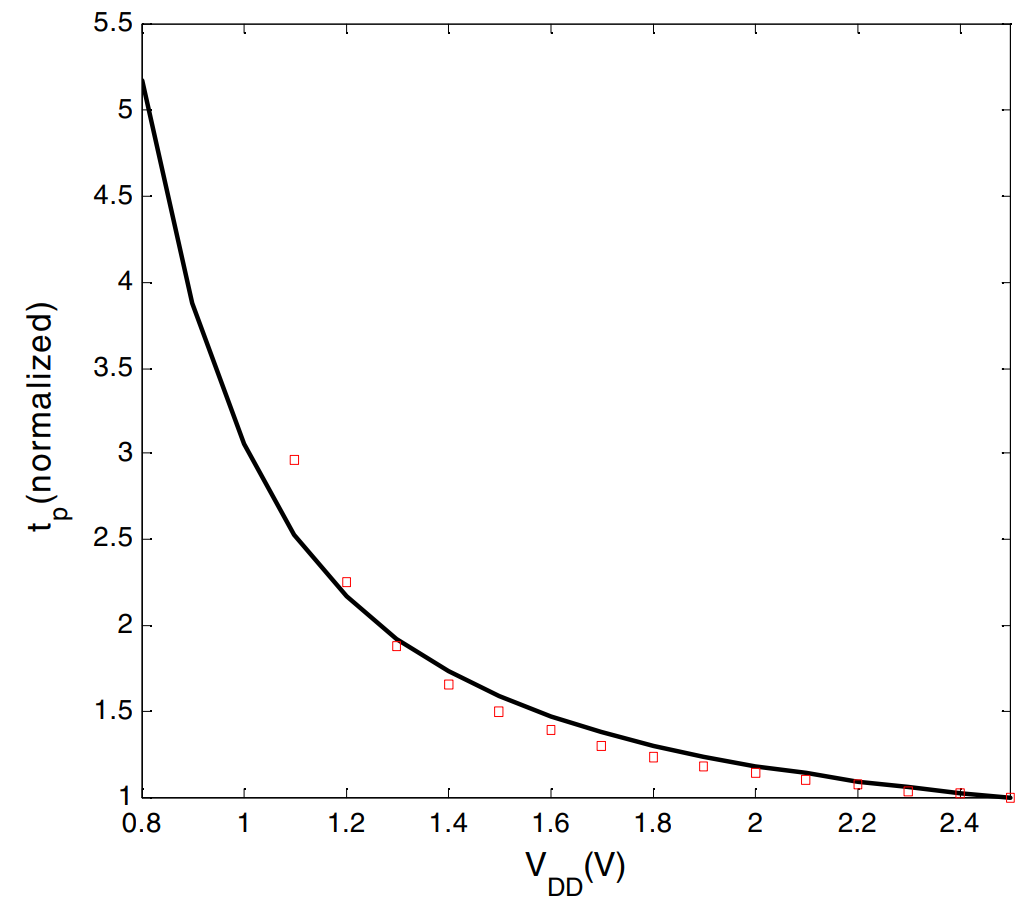
\includegraphics[width=0.45\linewidth]{img/ritardo_vdd.png}
    \caption{Simulazione di un ritardo di un transistore normalizzato}    
\end{figure}

Man mano che diminuiamo la tensione di alimentazione, aumenta notevolmente il ritardo: a $1.5\,V$ rispetto a $2.5\,V$ aumentiamo il ritardo del $50\%$.


\subsection{Teniamo conto di $V_{DD}$}

Possiamo tentare, in modo approssimato, di ricavare una formula che tiene conto di $V_{DD}$.

Corrente di	scarica in	saturazione è costante (non	siamo in	realtà	sempre	in	saturazione!):

\begin{equation*}
    I_D = \frac{1}{2}K_n(\vgs - \vtn)^2
\end{equation*}
\newpage
Dove $V_{GS} = V_{DD}$
\paragraph{}
Il tempo di propagazione lo abbiamo definito come il tempo che passa dal $50\%$ e per calcolarlo sulla $V_{DS}$ notiamo che siamo ancora abbastanza in saturazione. Quindi la corrente è abbastanza costante durante tutto il primo  $50\%$.

\begin{figure}[htbp]
    \centering
    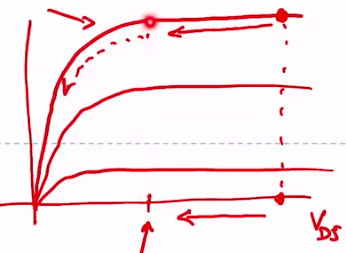
\includegraphics[width=0.37\linewidth]{img/saturaztion.png}
    \caption{$50\%$ di $V_{DS}$}    
\end{figure}

Quanto impieghiamo per scaricare l'uscita da $V_{DS}$ a $V_{DS}/2$?

\begin{equation*}
    I_D \cdot t_{PHL} = \frac{Q}{2} = \frac{1}{2}C\cdot\vdd
\end{equation*}
\begin{equation*}
    t_{pHL} = \frac{C\cdot\vdd}{K_n(\vgs - \vtn)^2} = \frac{C\cdot\vdd}{K_n(\vdd - \vtn)^2}
\end{equation*}


\paragraph{Esempi:} dato $C=10pF,\,K_n = 500 \,\mu A/V^2$

\begin{enumerate}
    \item $@3.3 \to 9 \,ns$
    \item $@2.5 \to 13.8\, ns$
    \item $@1.8\to 25\, ns$
\end{enumerate}

Se avessimo usato la formula che non teneva in considerazione il cambiamento della tensione in ingresso avremmo avuto:

\begin{equation*}
    t_{pHL} = \frac{0.63C}{K_n} = 12.6 \,ns
\end{equation*}

Altrimenti si fanno delle simulazioni con i vari Spice.

\section{Saturazione di velocità}
Un altro effetto di cui occorrerebbe tenere contro, soprattutto con la miniaturizzazione attuale, è che vi è una saturazione di velocità ovvero che si entra in saturazione molto prima. Dunque questa saturazione riduce la corrente di carica e scarica, i ritardi peggioreranno.

\subsection{Calcolo di resistenza media}
Consideriamo il tratto tra $V_{DD}$ e	$V_{DD}/2$	per	quanto riguarda il tempo	di	ritardo, non è possibile usare la $R_{on}$, utilizzata per quando $V_{DD}$ è nulla.

\begin{equation*}
    R_{eq} = \frac{1}{2}\biggl( \frac{\vdd}{I_{DSAT}(1+\lambda \vdd)} + \frac{V_{DD}/2}{I_{DSAT}(1+\lambda \vdd /2)} \biggl) = \frac{3}{4}\frac{\vdd}{I_{DSAT}}\biggl(1-\frac{5}{6}\lambda \vdd \biggl)
\end{equation*}

\begin{equation*}
    I_{DSAT} = K_n' \frac{W}{L}\biggl(\vdd - \vt - \frac{V_{SAT}}{2}\biggl)V_{SAT}
\end{equation*}
\newpage
Minore è il valore di	$V_{SAT}$,	minore è la	corrente $I_{DSAT}$,	e	maggiore
sarà la	resistenza equivalente.


\begin{figure}[htbp]
    \centering
    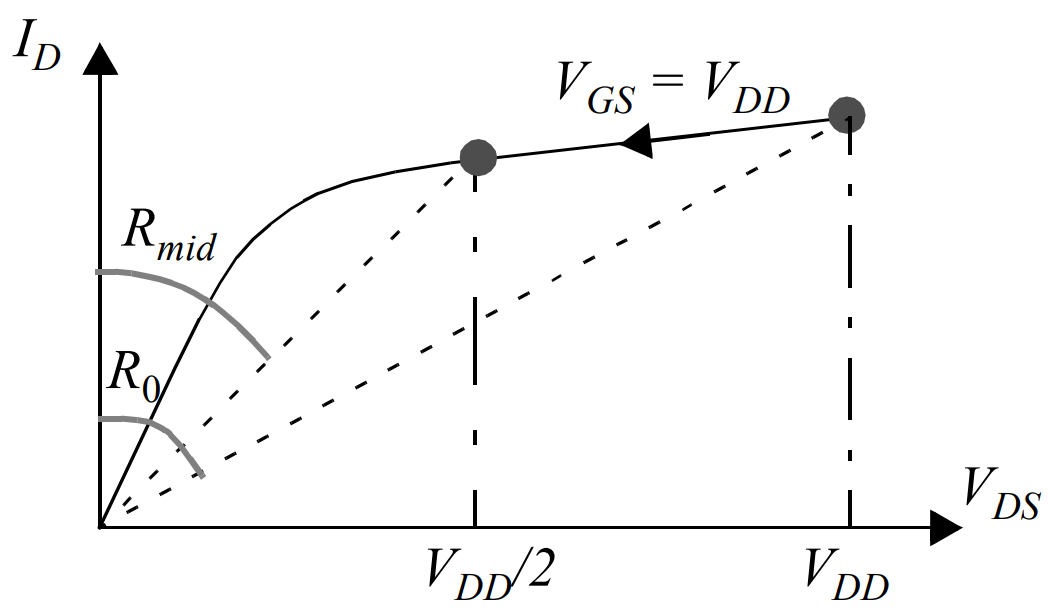
\includegraphics[width=0.5\linewidth]{img/R-onne.png}    
    
\end{figure}

L'inclinazione delle dure rette che collegano l'origine ai punti sopra indicati, è una resistenza.


\section{Consumo di potenza statico}

Le	porte CMOS	non	presentano un	consumo statico, dovuta all'uscita, di	potenza come	nel caso dell'inverter nMOS, questo significa che se la porta non sta facendo transizioni, non c'è un cammino da $V_{DD}$ a massa e dunque nessun consumo.

Però, come nel caso di una logica a rapporto, non vi è solo questo fattore di consumo statico bensì:

\begin{itemize}
    \item stiamo lavorando con componenti reali e il consumo vi è sempre solamente dall'uso dei fili;
    \item nei diodi tra drain/source e substrato vi è una corrente di polarizzazione inversa, moltiplicata per milioni di dispositivi diventa una corrente non irrisoria;
    \item Correnti dovute ad	effetti del	secondo	ordine,	quali la	conduzione sotto soglia;
    \item Correnti tra l'n-well	dei pMOS e	il substrato di	tipo p.
\end{itemize}

Consumo comunque molto	ridotto rispetto alla tecnologia nMOS, ecco perché molto usata questa logica CMOS.

\section{Consumo di potenza dinamico}

Unico consumo significativo per i dispositivi CMOS, dovuto all'energia necessaria per	caricare e	scaricare la	
capacità presente all'uscita. Ha	luogo solo	durante le	transizioni delle porte logiche.


\begin{figure}[htbp]
    \centering
    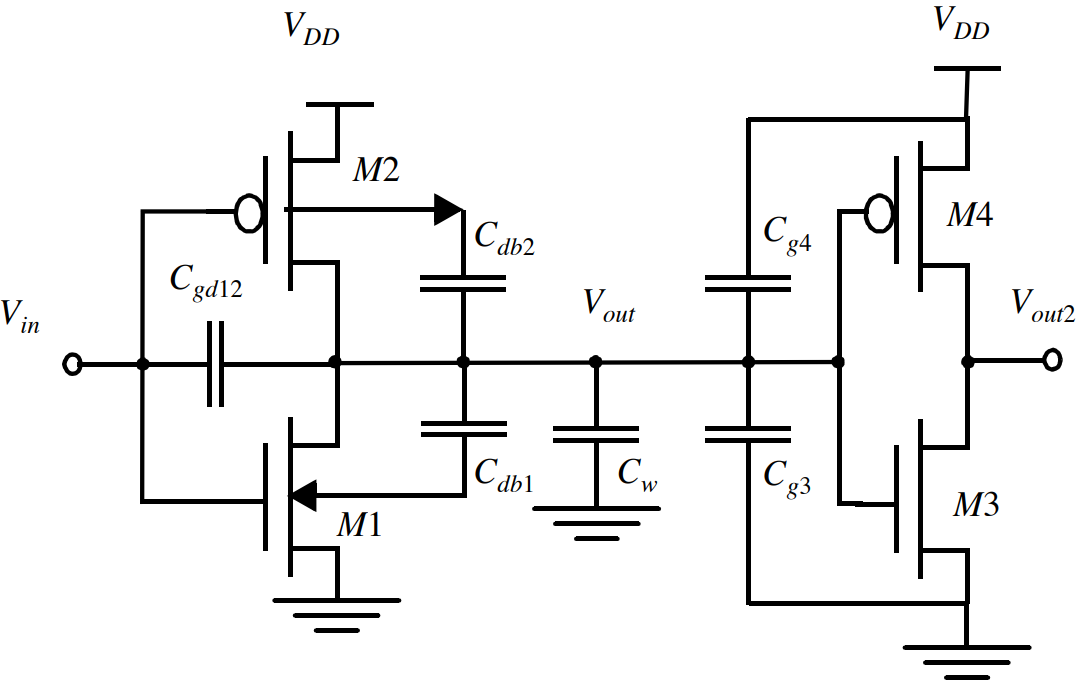
\includegraphics[width=0.5\linewidth]{img/cmosd.png}    
    
\end{figure}


\newpage
Capacità dovuta a	vari fattori

\begin{itemize}
    \item Capacità tra il drain	e	il gate;
    \item Capacità di	diffusione della giunzione p-n	del	drain;
    \item Capacità di	gate	delle porte a	valle;
    \item Capacità dei collegamenti.
\end{itemize}

Assumiamo	che inizialmente la	capacità sia scarica e al	tempo	t	=	0	l'interruttore si chiude e il	pMOS carica tramite la	sua resistenza interna il condensatore:

\begin{equation*}
    E_D = \int_0^\infty P(t)dt
\end{equation*}

La potenza è:

\begin{equation*}
    P(t) = V_{DD}I(t)
\end{equation*}

essendo $V_{DD}$ costante possiamo riscrivere la formula precedente:

\begin{equation*}
    E_D = V_{DD} \int_0^\infty I(t)dt
\end{equation*}


\begin{figure}[htbp]
    \centering
    \includegraphics[width=0.5\linewidth]{img/potenza:_dunb.png}
    
    
\end{figure}

La	corrente è quella che scorre nel condensatore:

\begin{equation*}
    I(t) = C\frac{dV}{dt}
\end{equation*}

Sostituendo a $E_D$:

\begin{equation*}
    E_D = V_{DD} \int_0^\infty C\frac{dV}{dt}dt = CV_{DD} \int_{V_C(o)}^{V_C(\infty)} dV_c
\end{equation*}

Con le condizioni a contorno messe precedentemente: $V_C(0) = 0\,V$ e $V_C(\inf) = V_{DD}$

\begin{equation*}
    E_D = CV_{DD}^2
\end{equation*}

L'energia immagazzinata in C è

\begin{equation*}
    \varepsilon_s = \frac{1}{2}CV_{DD}^2
\end{equation*}

mentre l'energia dissipata risulta essere:

\begin{equation*}
    \varepsilon_l = CV_{DD}^2 - \frac{1}{2}V_{DD}^2 = \frac{1}{2}V_{DD}^2
\end{equation*}

Dunque \textbf{solo metà dell'energia} donata dal generatore ha effettivamente caricato il condensatore, l'altra metà è stata dissipata dal transistore e dai collegamenti.

\newpage
\paragraph{Ora facciamo il contrario, scarichiamo la capacità}

L'energia	$\varepsilon_s $ immagazzinata nel condensatore viene dissipata nella transizione contraria, pertanto l'energia totale dissipata in una transizione completa allora è:


\begin{equation*}
    \varepsilon_{TD} = \varepsilon_l  + \varepsilon_s = \frac{1}{2}CV_{DD}^2 + \frac{1}{2}CV_{DD}^2 = CV_{DD}^2
\end{equation*}

La	potenza dissipata equivale all'energia nell'unità di	tempo, se	la	porta	commuta con	frequenza f (transizioni complete nell'unità di tempo):

\begin{equation*}
    P_D = CV_{DD}^2f\alpha
\end{equation*}

Dove:

$\alpha = $ fattore di attività [0 (segnale costante), 1 (segnale che commuta ad ogni ciclo)]

\paragraph{}

Più è elevata la capacità e più si consuma, da notare che la tensione compare come termine al quadrato, questo significa che diminuendo la tensione di alimentazione consumeremo molto meno. Diminuendola di metà consumeremo quattro volte in meno, ecco le continue diminuzioni di tensione di alimentazione nei circuiti moderni, ma non troppo dato che vi è il trade-off con le prestazioni (diminuzione di tensione di alimentazione: consumi minori, ma prestazioni peggiori).


\begin{figure}[htbp]
    \centering
    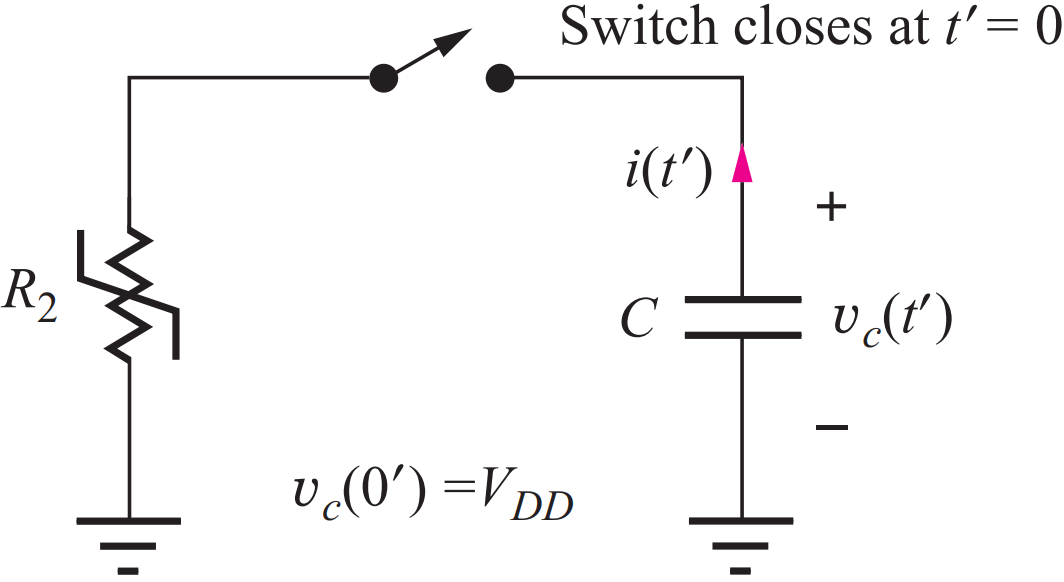
\includegraphics[width=0.5\linewidth]{img/adlsocn.png}
    
    
\end{figure}

La potenza dunque dipende da:

\begin{itemize}
    \item frequenza di	commutazione
    \item capacità di	carico (architettura)
    \item quadrato della tensione di alimentazione
\end{itemize}

\paragraph{NOTA:} ad ogni glitch del circuito avremo una transizione completa.

\paragraph{Circuiti adiabatici:} si vede come il ciclo di carica è efficiente solo per il 50\%, ci sono dei circuiti chiamati circuiti adiabatici che provvedono a recuperare il calore speso e trasformarlo in lavoro. Circuiti molto difficili da costruire.

\newpage
\section{Corrente di corto circuito}

Il	segnale di	ingresso non	passa da	0	a	$V_{DD}$ istantaneamente, infatti i due transistor in questa fase sono in conduzione entrambi. In questo periodo vi è un passaggio di corrente tra $V_{DD}$ e massa che non contribuisce al caricamento della capacità. 

Questo valore di corrente che viene buttata può arrivare fino a valori del 20-30\% di quella necessaria per scaricare la capacità. Anche questo inciderà sul consumo di potenza effettivo. Tutto questo dipende dal dimensionamento dei transistori e da quanto vanno veloci i transistori a monte.

\begin{figure}[htbp]
    \centering
    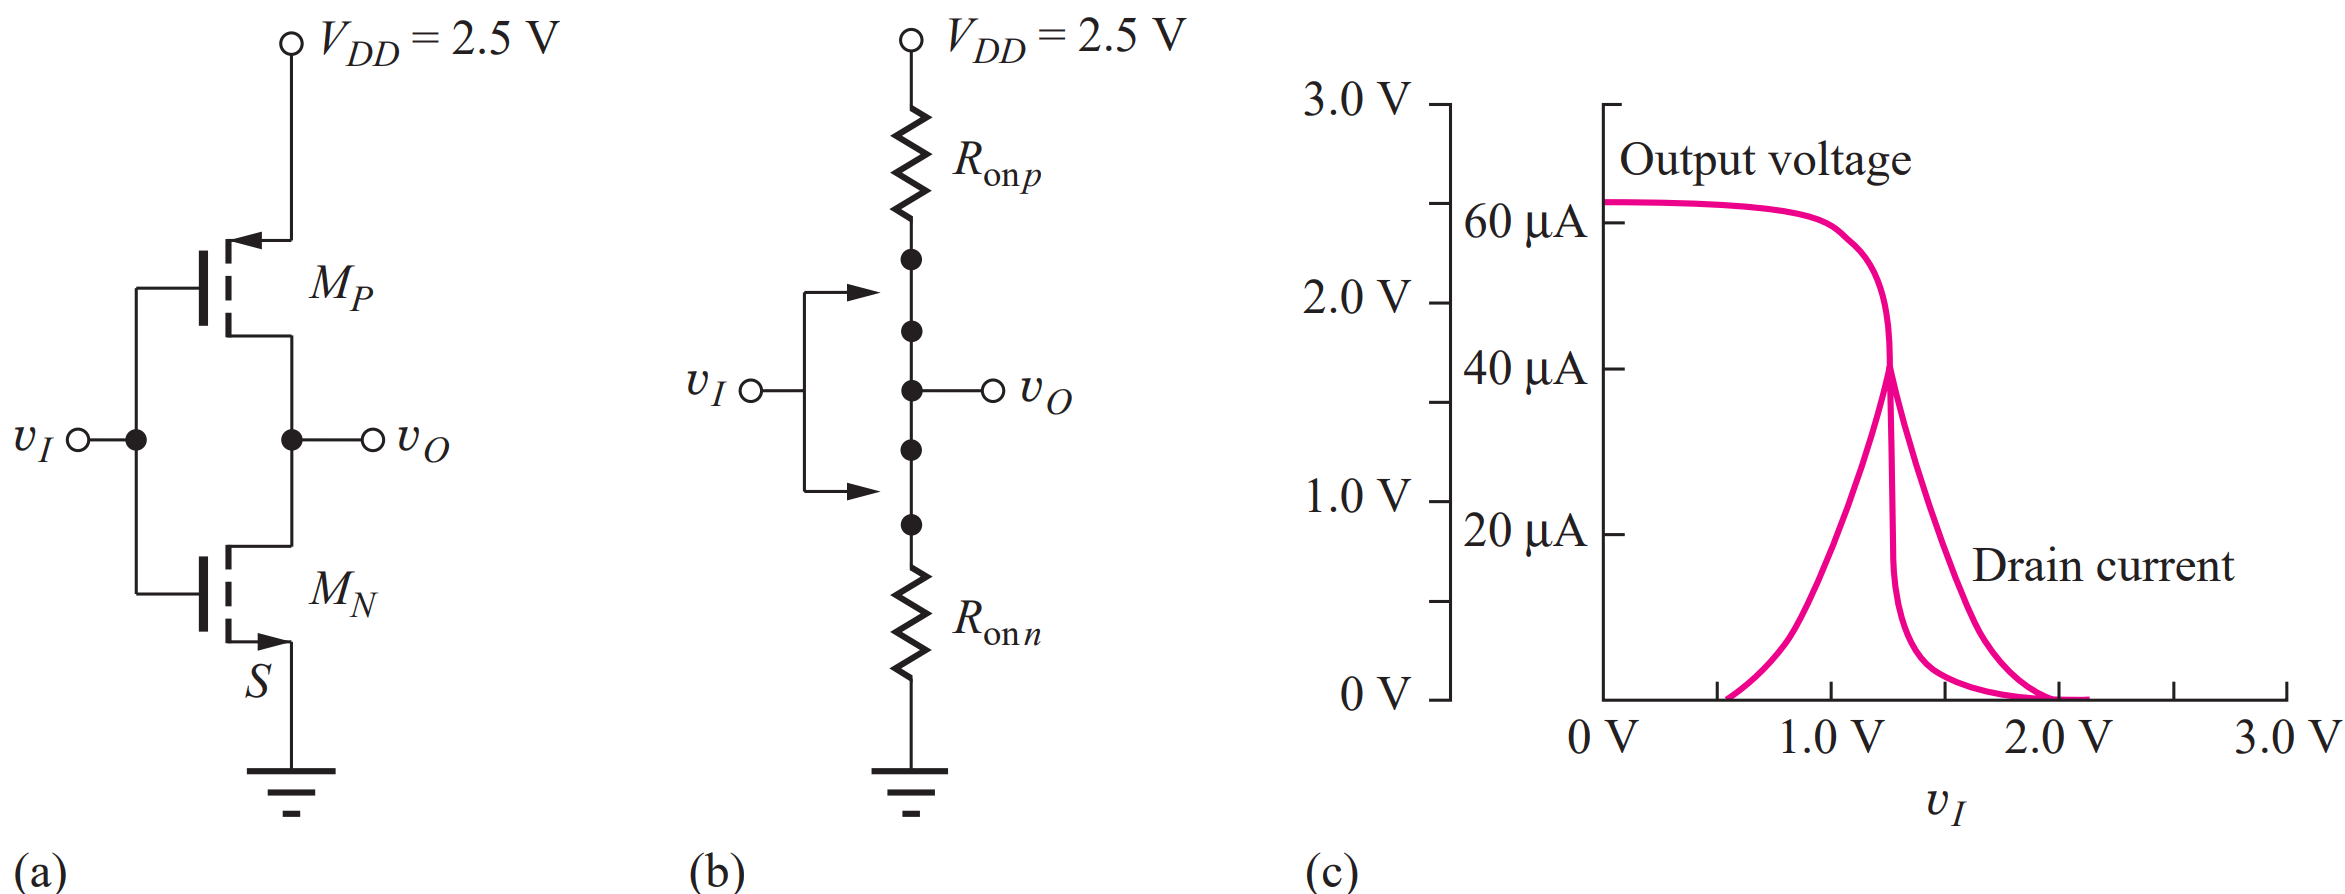
\includegraphics[width=0.9\linewidth]{img/non_step_ingresso.png}
\end{figure}


\section{Compromessi}

\begin{itemize}
    \item Area: in CMOS possiamo fare transistori piccoli, ciò comporta ad una scarsa conduzione di corrente;
    \item Consumi: ridurre la tensione di alimentazione, e in concomitanza anche la frequenza (altrimenti si produrrebbero errori), porta a consumi minori, scarse prestazioni. Riduzione di C;
    \item Margini di rumore: transitori bilanciati (area non minima), tensione di alimentazione alta;
    \item Prestazioni: transistori grandi, tensione di alimentazione alta
\end{itemize}


\begin{figure}[htbp]
    \centering
    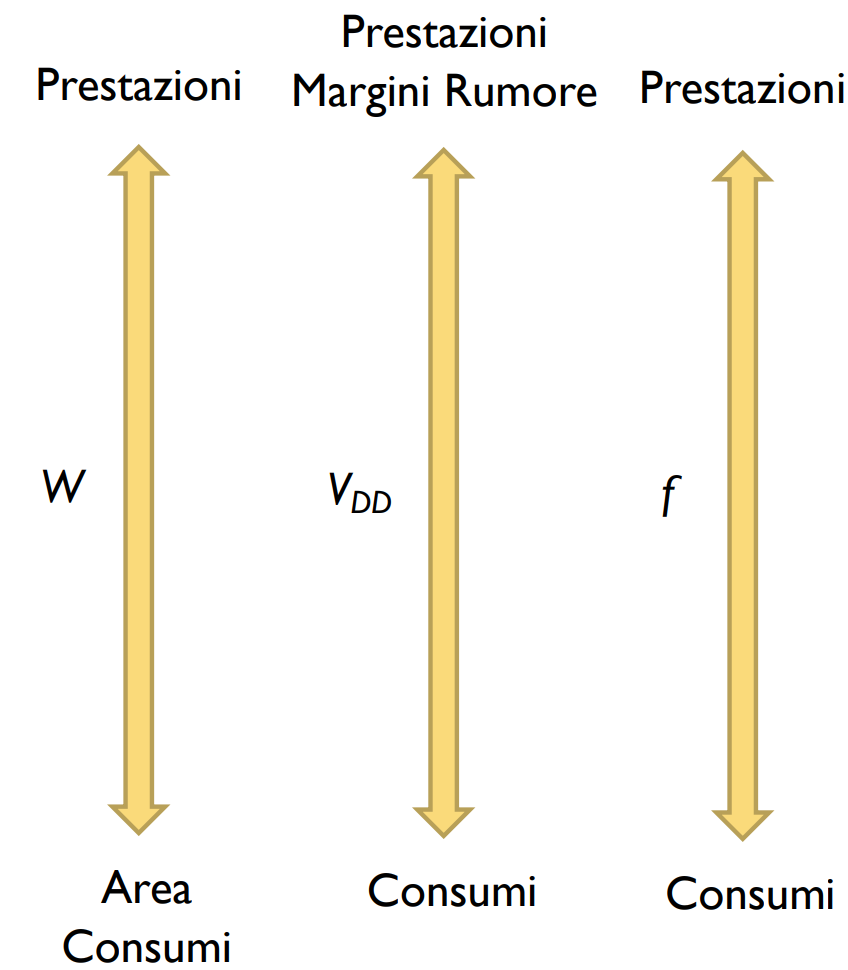
\includegraphics[width=0.3\linewidth]{img/comporomessi.png}
\end{figure}

\newpage
\section{Costruzione di porte logiche}

Come abbiamo visto per l'inverter, il pull-up e il pull-down dovranno essere sostanzialmente simmetrici, appunto complementari. Non	dovranno mai condurre contemporaneamente, se una ha una connessione in serie, l'altra è in parallelo, e viceversa.


\subsubsection{Esempio della NAND}

\begin{figure}[htbp]
    \centering
    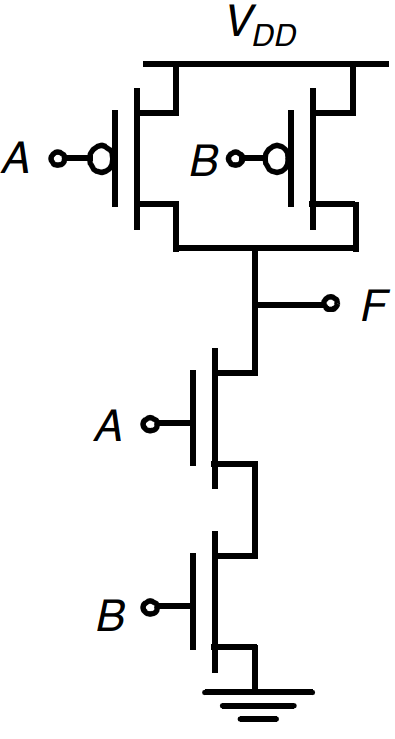
\includegraphics[width=0.17\linewidth]{img/NAND_CMOS.png}
    \caption{NAND in logica CMOS}    
\end{figure}


\subsubsection{Esempio della NOR}

\begin{figure}[htbp]
    \centering
    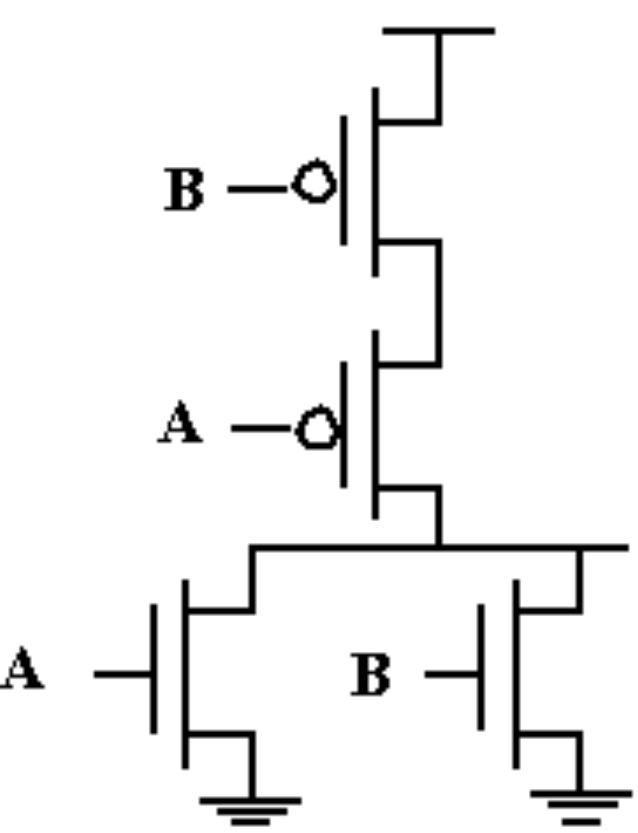
\includegraphics[width=0.2\linewidth]{img/NOR_CMOS.png}
    \caption{NOR in logica CMOS}     
\end{figure}

\newpage

\paragraph{Realizzare	la	funzione		F	=	(D	+	A ·	(B	+	C))'}

\paragraph{}
\begin{figure}[htbp]
    \centering
    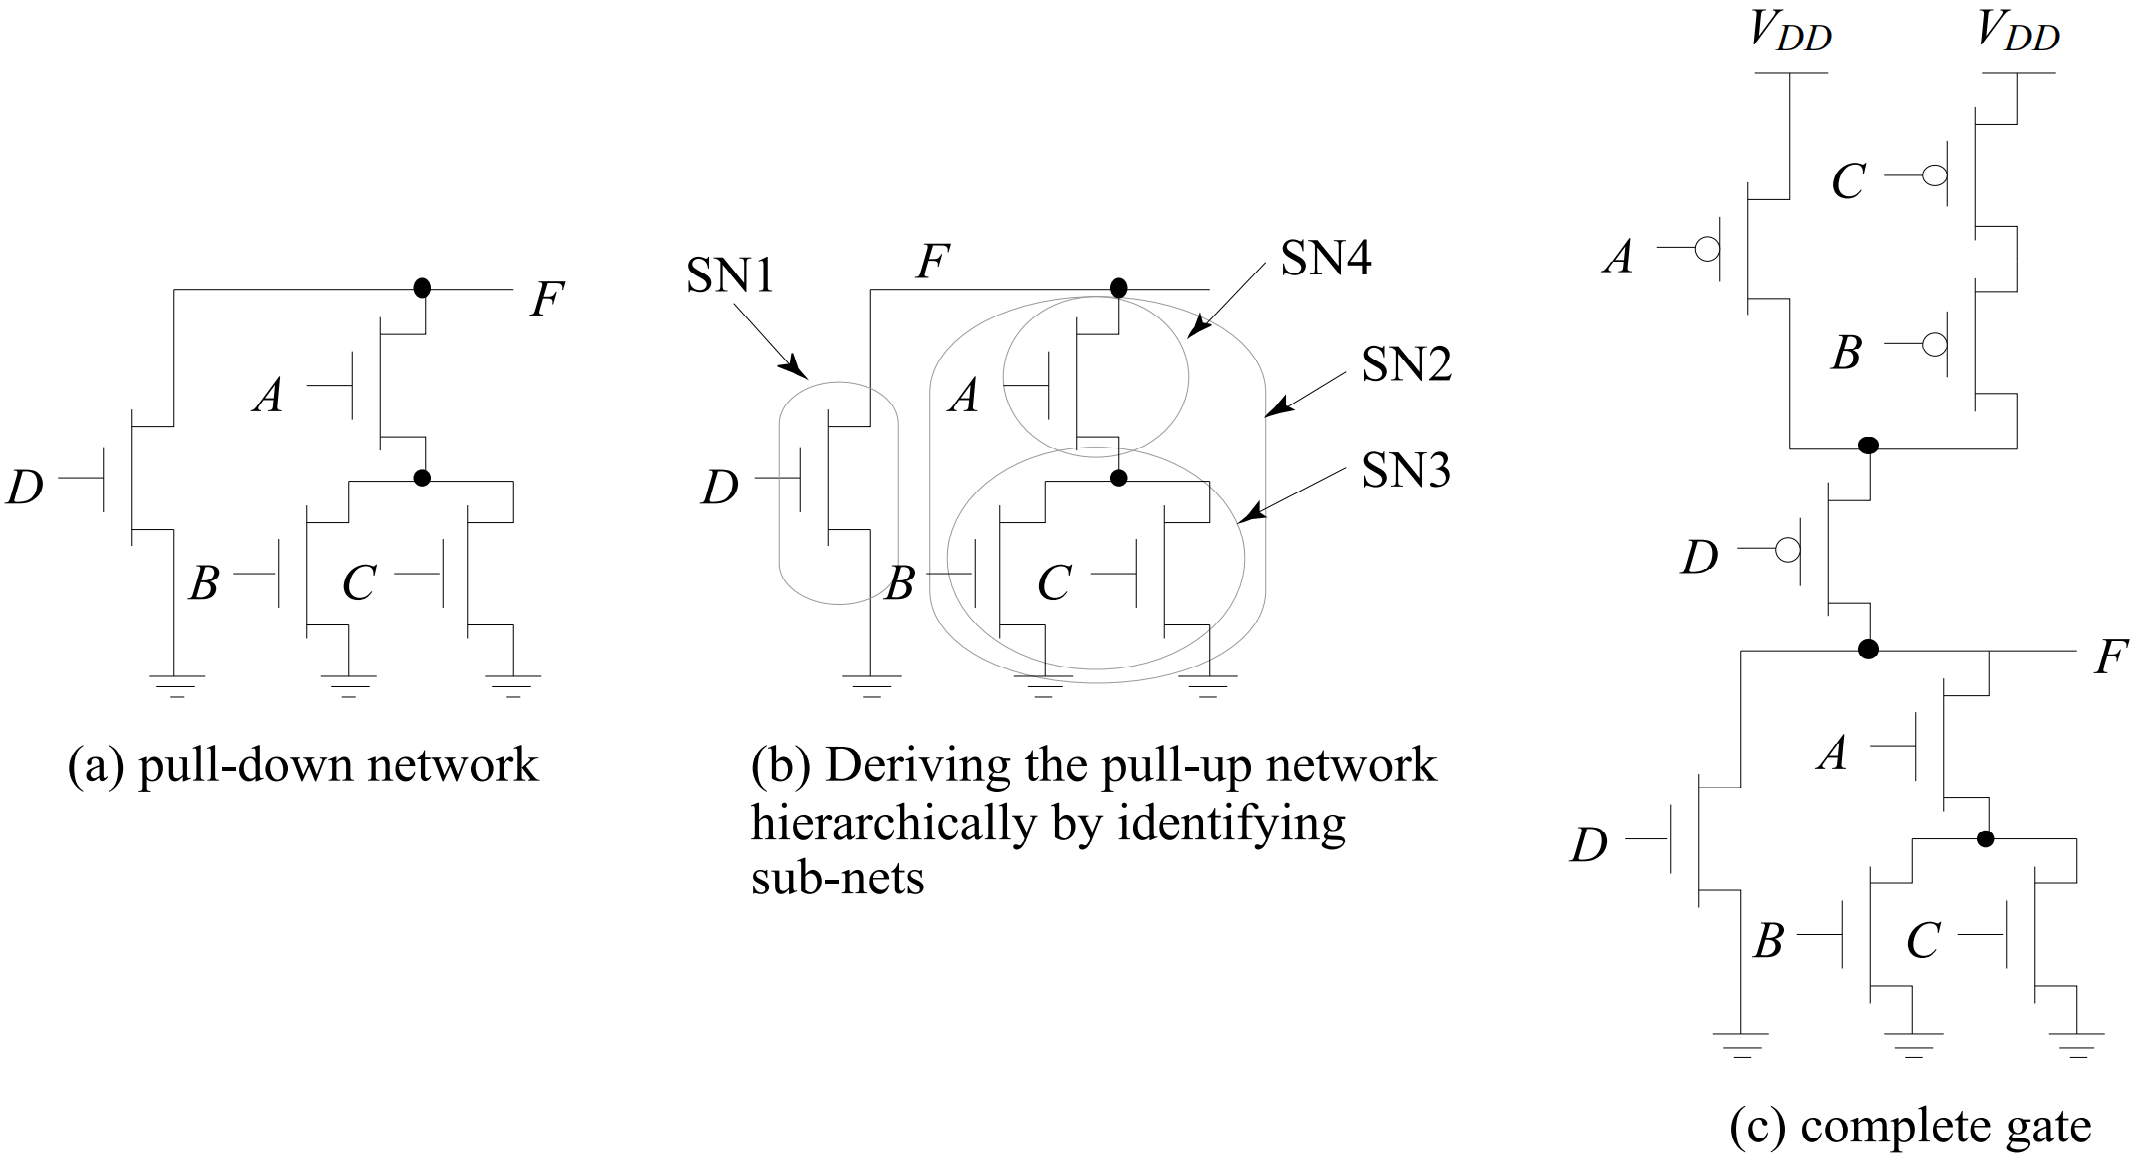
\includegraphics[width=0.8\linewidth]{img/rete.png}   
    
\end{figure}

\paragraph{NOTA:}

\begin{itemize}
    \item Ogni	variabile	che	appare	nella	formula	dà	luogo	a	due	transistori;
    \item Se	una	variabile	appare	più	volte,	darà	luogo	ad	altrettante	coppie	di	transistori;
    \item Costa di più in quanto è più grosso di una logica a nMOS, questo però si recupera in termini di potenza.
    
\end{itemize}

\newpage
\section{Dimensionamento dei transistori}

In questo caso non è necessario per	i livelli di	uscita, infatti l'output	range	sempre tra  0V	e	$V_{DD}$, ma è utile per determinare i ritardi, infatti verranno dimensionati per i valori di ritardo che vogliamo ottenere.

Per fare ciò possiamo usare le formule già viste in precedenza, infatti il ritardo è inversamente proporzionale al rapporto $W/L$.

\begin{equation}
    R_{on} = \frac{1}{K_n'\frac{W}{L}(V_{GS} - V_{TN})}
\end{equation}

oppure usando un il modello che utilizza la velocità di saturazione:

\begin{equation*}
    R_{eq} = \frac{1}{2}\biggl(\frac{V_{DD}}{I_{DSAT}(1+\lambda V_{DD})} + \frac{V_{DD}/2}{I_{DSAT}(1+\lambda V_{DD}/2)}\biggl)
\end{equation*}

dove

\begin{equation*}
    I_{DSAT} = K_n' \frac{K}{L}\biggl(V_{DD} - V_T - \frac{V_{SAT}}{2}\biggl)V_{SAT}
\end{equation*}

Si prenda a	riferimento un	inverter,	e	si considerano i casi peggiori, considerando $K_n' = 2.5 K_p'$ mantenendo dei ritardi simmetrici:

\begin{figure}[htbp]
    \centering
    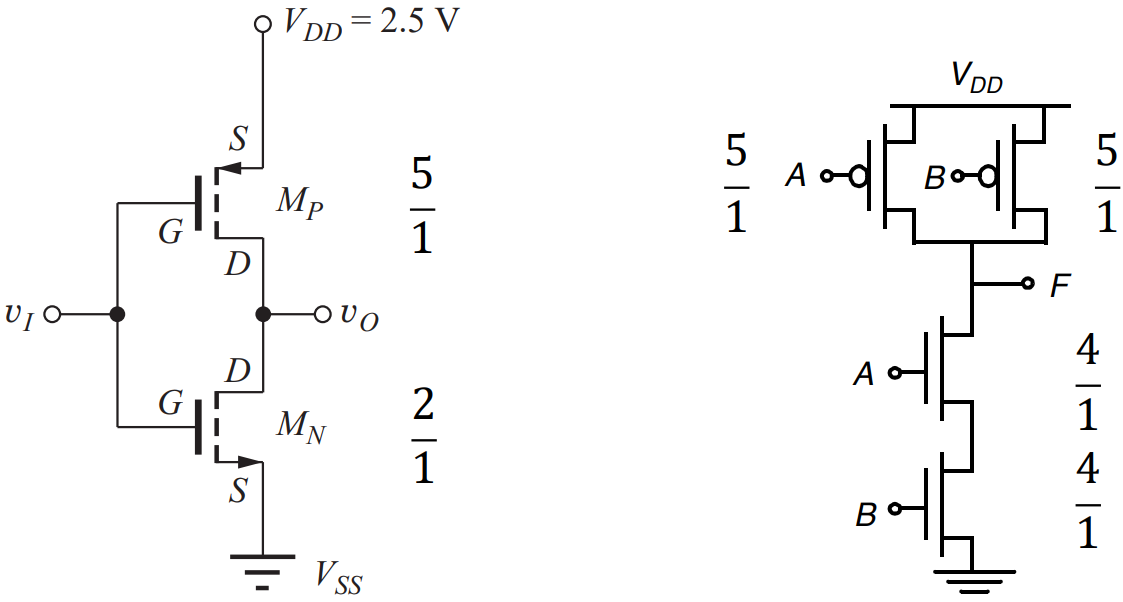
\includegraphics[width=0.7\linewidth]{img/dimensionamento.png}
\end{figure}


\begin{figure}[htbp]
    \centering
    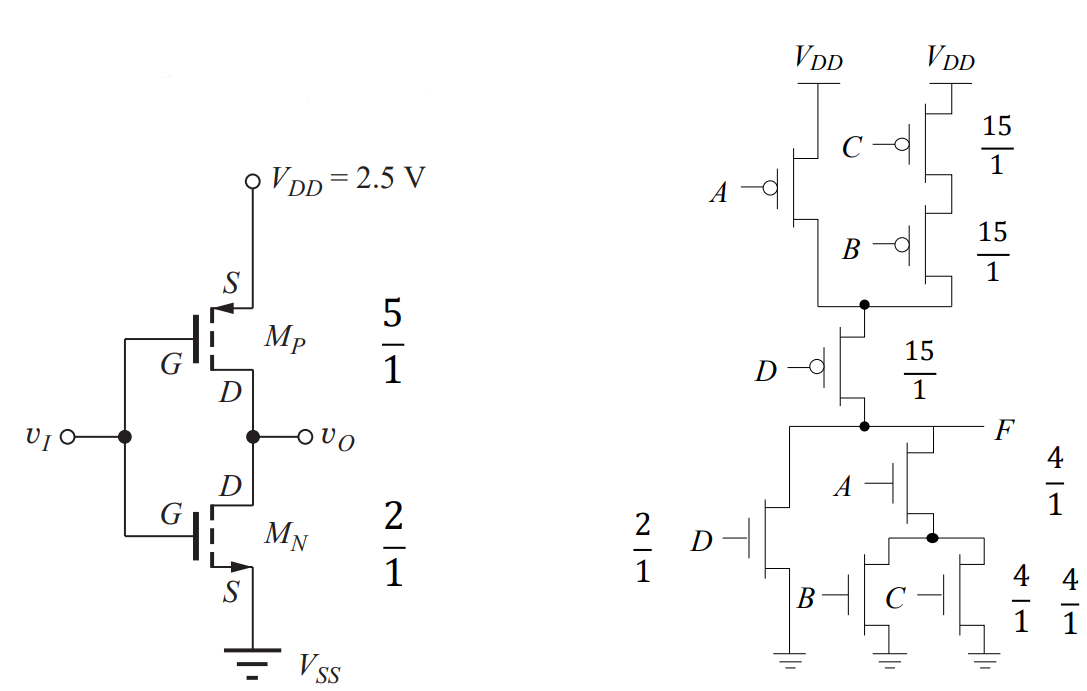
\includegraphics[width=0.75\linewidth]{img/dim_cmos.png}   
    
\end{figure}


\newpage
Per l'ultimo pMOS si assuma che $R_{on}$ sia la resistenza di un transistor 1/1. Per	un	transistor	di	dimensione W/L	la	
resistenza equivalente sarà:

\begin{equation*}
    R_{eq} = \frac{R_{on}}{\frac{W}{L}}
\end{equation*}

Per la serie vogliamo che:

\begin{equation*}
    \frac{R_{on}}{\frac{W}{L}}_D + \frac{R_{on}}{\frac{W}{L}}_A = \frac{R_{on}}{\frac{5}{1}} \to \frac{R_{on}}{\frac{15}{1}}_D + \frac{R_{on}}{\frac{W}{L}}_A = \frac{R_{on}}{\frac{5}{1}}
\end{equation*}

\begin{equation*}
    1+ \frac{15}{\frac{W}{L}}_A = 3 \to \frac{W}{L}_A = 7.5
\end{equation*}


\section{Take away}

\begin{itemize}
    \item Margini di	rumore elevati: le	uscite	sfruttano	l'intero	range	di	valori,	da	0	a	$V_{DD}$, inoltre i	livelli	 logici	non	dipendono	dal	rapporto	di	dimensione	dei	transitori,	e	sono	ripristinati	ad	ogni	porta	logica;
    \item Alta	impedenza	di	ingresso,	bassa	impedenza	di	uscita, semplifica	l'accoppiamento	tra	stadi	successivi;
    \item Consumi di	potenza statici ridotti nulli se	non	si considera la	corrente di	leakage;
    \item Tempi	di	salita e	discesa equivalenti e	facilmente controllabili, occorre dimensionare opportunamente i	transistori per	compensare la	 differenza di	mobilità	tra	transistori	n e	p;
    \item Alta	occupazione	di	area,  richiede	una	coppia	di	transitori	per	ogni	ingresso.
\end{itemize}

